\chapter{Report and analysis}

\section{Project structure}
\tikzset{every picture/.style={line width=0.75pt}} 
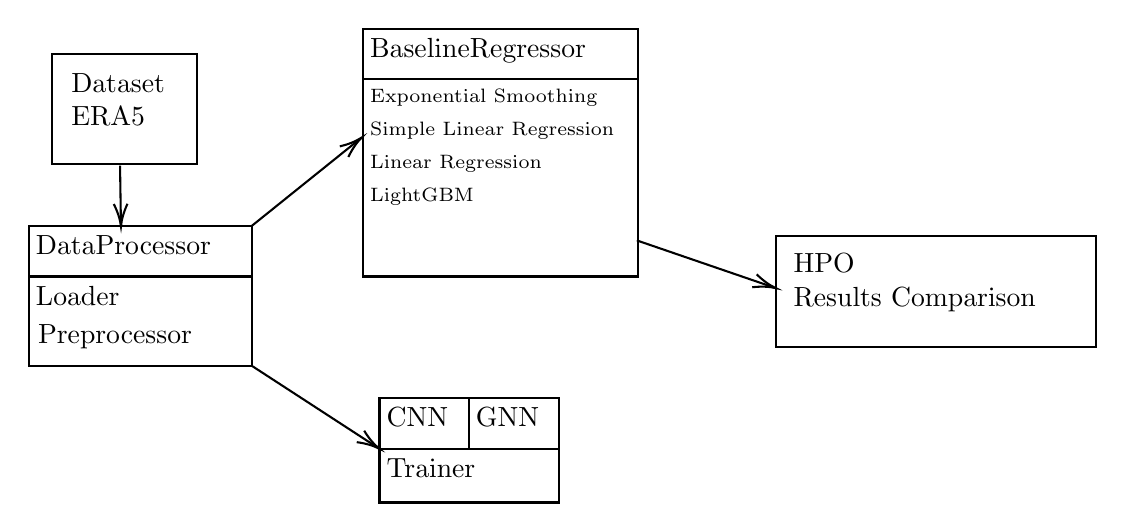
\begin{tikzpicture}[x=0.75pt,y=0.75pt,yscale=-1,xscale=1]
\draw   (49,24) -- (119,24) -- (119,77.4) -- (49,77.4) -- cycle ;
\draw   (38,107) -- (145.47,107) -- (145.47,131.4) -- (38,131.4) -- cycle ;
\draw   (199,12) -- (331.47,12) -- (331.47,36.4) -- (199,36.4) -- cycle ;
\draw   (38,131.4) -- (145.47,131.4) -- (145.47,174.4) -- (38,174.4) -- cycle ;
\draw   (199,36.4) -- (331.47,36.4) -- (331.47,131.4) -- (199,131.4) -- cycle ;
\draw    (82,78) -- (82.42,105.35) ;
\draw [shift={(82.45,107.35)}, rotate = 269.12] [color={rgb, 255:red, 0; green, 0; blue, 0 }  ][line width=0.75]    (10.93,-3.29) .. controls (6.95,-1.4) and (3.31,-0.3) .. (0,0) .. controls (3.31,0.3) and (6.95,1.4) .. (10.93,3.29)   ;
\draw    (145.47,107) -- (196.91,65.65) ;
\draw [shift={(198.47,64.4)}, rotate = 141.21] [color={rgb, 255:red, 0; green, 0; blue, 0 }  ][line width=0.75]    (10.93,-3.29) .. controls (6.95,-1.4) and (3.31,-0.3) .. (0,0) .. controls (3.31,0.3) and (6.95,1.4) .. (10.93,3.29)   ;
\draw   (207,190) -- (293.47,190) -- (293.47,214.4) -- (207,214.4) -- cycle ;
\draw   (207,214.4) -- (293.47,214.4) -- (293.47,240.27) -- (207,240.27) -- cycle ;
\draw    (250.1,190.17) -- (250.1,214.17) ;
\draw    (145.47,174.4) -- (205.32,213.31) ;
\draw [shift={(207,214.4)}, rotate = 213.03] [color={rgb, 255:red, 0; green, 0; blue, 0 }  ][line width=0.75]    (10.93,-3.29) .. controls (6.95,-1.4) and (3.31,-0.3) .. (0,0) .. controls (3.31,0.3) and (6.95,1.4) .. (10.93,3.29)   ;
\draw   (398,112) -- (552,112) -- (552,165.4) -- (398,165.4) -- cycle ;
\draw    (331,114) -- (396.11,136.35) ;
\draw [shift={(398,137)}, rotate = 198.95] [color={rgb, 255:red, 0; green, 0; blue, 0 }  ][line width=0.75]    (10.93,-3.29) .. controls (6.95,-1.4) and (3.31,-0.3) .. (0,0) .. controls (3.31,0.3) and (6.95,1.4) .. (10.93,3.29)   ;
\draw (57,32) node [anchor=north west][inner sep=0.75pt]   [align=left] {Dataset\\ERA5};
\draw (40,110) node [anchor=north west][inner sep=0.75pt]   [align=left] {DataProcessor};
\draw (40,134.4) node [anchor=north west][inner sep=0.75pt]   [align=left] {Loader};
\draw (41,153) node [anchor=north west][inner sep=0.75pt]   [align=left] {Preprocessor};
\draw (201,15) node [anchor=north west][inner sep=0.75pt]   [align=left] {BaselineRegressor};
\draw (201,39.4) node [anchor=north west][inner sep=0.75pt]   [align=left] {{\scriptsize Exponential Smoothing}\\{\scriptsize Simple Linear Regression}\\{\scriptsize Linear Regression}\\{\scriptsize LightGBM}};
\draw (209,193) node [anchor=north west][inner sep=0.75pt]   [align=left] {CNN \ \ GNN};
\draw (209,217.4) node [anchor=north west][inner sep=0.75pt]   [align=left] {Trainer};
\draw (405,119) node [anchor=north west][inner sep=0.75pt]   [align=left] {HPO \\Results Comparison};
\end{tikzpicture}

\section{Dataset description}\label{chap:dataset}
Description of dataset, train, val, test split, resoution of data, generally all details.
\begin{itemize}
    \item Motivation behind usage of GRIB files and their description.
\end{itemize}

\section{Preprocessing methods}
Dividing time series into window sequences, normalization techniques

\section{Experiments}

\subsection{Hyperparameters optimization}
A short definition of Bayesian optimization and presentation of used Optuna sampler - Tree-Structured Parzen Estimator.~\cite{watanabe2023treestructured} 

\section{Results}
Results presentation, comparision with other models/benchmark scores. Visualisation and analysis.

\section{Practical details}
Explain training, evaluating and forecasting details and methods - e.g. spatial mapping of neural nets;
normalization and regularization techniques, used metrics and objectives, post processing, computation time, software and hardware stack etc. 
